\documentclass[11pt,a4paper]{article}
\usepackage[T1]{fontenc}
\usepackage[margin=1in]{geometry}
\usepackage{amsmath,amssymb,amsthm,mathtools}
\usepackage{booktabs}
\usepackage{xcolor}
\usepackage[colorlinks=true,linkcolor=blue!60!black,citecolor=blue!60!black,
            urlcolor=blue!60!black]{hyperref}
\usepackage{microtype}
\usepackage{enumitem}
\usepackage{graphicx}
\usepackage[most]{tcolorbox}

\newcommand{\lean}[1]{\texttt{\small #1}}
\newtcolorbox{keybox}[1][]{colback=blue!3,colframe=blue!45!black,
  boxrule=0.5pt,left=4pt,right=4pt,top=3pt,bottom=3pt,#1}
\newtcolorbox{failbox}[1][]{colback=red!3,colframe=red!45!black,
  boxrule=0.5pt,left=4pt,right=4pt,top=3pt,bottom=3pt,#1}
\newtheorem{theorem}{Theorem}
\newcommand{\PENDING}{\textcolor{red}{[pending]}}

\title{\textbf{Topological sectors carry their own temperature}\\
\large A proposal: a machine-checked mediant theorem, a torus vortex thermometer with its known answers,\\
the data that can test the hypothesis, and what would kill it}

\author{Xavier Callens\\
\small SocrateAI-Scientific-QuantumFluids\\
\small \url{https://github.com/xaviercallens/SocrateAI-Scientific-QuantumFluids}}
\date{September 2026 -- proposal; predictions fixed before the runs}

\begin{document}
\maketitle

\begin{abstract}
\noindent
A pre-registered intervention on a two-dimensional Bose gas~\cite{Callens2026Causal} found that two
boxes with the same energy, particle number and momentum, one carrying four injected vortex pairs and one
carrying the same energy as phonons, read different temperatures on the same thermometer, the vortex box
being colder by $5$--$16\%$. We propose the reading that the literature on point-vortex matter has held
since Onsager~\cite{Onsager1949,KraichnanMontgomery1980} and that two experiments made
quantitative~\cite{Gauthier2019,Johnstone2019}: the vortex configuration is a subsystem with its own
temperature, weakly coupled to the phonon bath, and a thermometer that reads the bath reads one of two
temperatures. We state the hypothesis in a form that can fail, prove its combinatorial core in Lean~4
(the inverse temperature of a state that mixes sectors is a mediant of the sector inverse temperatures,
so equal energy does not imply equal temperature once a conserved label exists), build the instrument
that measures the second temperature on a torus (the Weiss--McWilliams point-vortex energy with its
published known answer, and a canonical Monte Carlo calibration after Groszek et al.), and list the data
that can test the hypothesis: our own runs with two thermometers, the public vortex-position data of
Gauthier et al., and the superfluid-density data of Christodoulou et al. Every prediction below is fixed
before the corresponding run or analysis. No physics is claimed as new.
\end{abstract}

\section{The observation and the hypothesis}

\paragraph{Observation (round 2 of~\cite{Callens2026Causal}).} On three equilibrated base states, arm V
(four imprinted vortex--antivortex pairs) and arm P (the same $\Delta E$ as random phonons, matched to
machine precision) were compared over $t\in[100,300)$. The condensate fell by $0.49$--$0.73$ in V and by at
most $0.035$ in P; the coherence exponent grew $9$--$44\times$ in V; and the two-window equipartition
thermometer read V colder than P by $5.5\%$, $9.2\%$ and $16\%$, and colder than the untouched base by
$4\%$, with total energy conserved to $2\times10^{-7}$. The pre-registered composite claim required equal
readings and was not made.

\paragraph{Hypothesis F.} The microcanonical entropy depends on the sector, $S(E,N,P,W)$, so
$1/T=\partial S/\partial E$ at fixed $W$ is sector-dependent. Concretely the field is a two-temperature
system: a phonon bath at $T_b$ and a vortex gas at $T_v=(\partial S_v/\partial E_v)^{-1}$ defined on the
vortex positions~\cite{Onsager1949}. Topological protection is the weak coupling that keeps $T_v\ne T_b$
for a long time. Injecting a configuration with $T_v\gg T_b$ (an imprinted arrangement near the
maximum-entropy energy of the vortex gas) draws energy from the bath into the vortex system as the
configuration relaxes towards its own equilibrium and nucleates further pairs; the bath cools.

\paragraph{What would kill it.} (K1) The torus vortex thermometer, calibrated canonically, fails its
closure test (set $\beta$, read $\beta$ back within $10\%$). (K2) On the V arm, $T_v$ and $T_b$ agree
within their errors from the first block on. (K3) The bath's energy loss is not matched, within $30\%$,
by the vortex system's energy gain over the same blocks. (K4) On the Gauthier data, the decay time of the
clustered configuration does not fall as the condensate fraction falls.

\section{The combinatorial core, machine-checked}

Let $\Omega$ be a finite set of microstates with energy level $\varepsilon:\Omega\to\mathbb N$ and sector
label $w:\Omega\to\mathbb Z$. Write $n_W(E)$ for the number of microstates in sector $W$ at energy $E$ and
$N(E)=\sum_W n_W(E)$. The discrete inverse-temperature factor of a sector is $e^{\beta_W}=n_W(E+1)/n_W(E)$
and the global one is $e^{\beta}=N(E+1)/N(E)$.

\begin{theorem}[\lean{SectorTemperature.globalRatio\_mem}]
If every occurring sector has $n_W(E)>0$ and $r_1\le e^{\beta_W}\le r_2$ for all $W$, then
$r_1\le e^{\beta}\le r_2$.
\end{theorem}
The proof is the mediant inequality for ratios of nonnegative sums; the file also proves $N=\sum_W n_W$,
$\log n_W\le\log N$, equality of the global and sector factors when a single sector is populated, and --
via the conservation theorem of~\cite{Callens2026Causal} -- that the sectors are invariant sets of every
continuous evolution without a phase slip, which is what makes $S(E,W)$ meaningful. Eight theorems,
standard axioms, three negative controls fail (mediant without positivity; global equal to an arbitrary
sector; the entropy inequality reversed). Comparator: accepted by the \lean{nanoda} kernel and by the Lean kernel (2026-09-25).

What the theorem says for the observation: a thermometer that does not know the sector reads a weighted
mean of sector temperatures, and two states of the same energy in different sectors need not share it.
What it does not say: which temperature the equipartition estimator reads on a continuum field. That is
an empirical question, and Section~\ref{sec:data} is how it is answered.

\section{The instrument and its known answers}

\paragraph{Torus point-vortex energy.} Weiss and McWilliams~\cite{WeissMcWilliams1991}, eq.~(12): on the
$2\pi$ box, $h(x,y)=\sum_m\ln[(\cosh(x-2\pi m)-\cos y)/\cosh 2\pi m]-x^2/2\pi$,
$H=-\sum_{i<j}\kappa_i\kappa_j h(\mathbf r_{ij})$, zero total circulation and zero vortex momentum.
Physical units here: $E_{\rm phys}=\pi E_{\rm WM}$, $\beta_{\rm phys}=\beta_{\rm WM}/\pi$ ($\rho=1$,
$\kappa=2\pi$). Known answers run before any reading: the dipole energy grows by $2\ln2$ per doubling of
the separation ($1.384$, $1.377$ measured; two-dimensional Coulomb); the density of states of six vortices
at zero momentum has rms $2.985$ against their $2.90$; the mean differs by an additive convention that a
temperature cannot see.

\paragraph{Canonical calibration.} Metropolis sampling at set $\beta$ with pair moves that conserve the
vortex momentum, for $N=4$ to $16$ vortices, giving $\langle E\rangle(\beta)$ and the dipole and cluster
fractions of Groszek et al.~\cite{Groszek2018}. Two internal checks: $d\langle E\rangle/d\beta=-{\rm Var}(E)$
at every interior grid point, and closure (K1). Results: \PENDING.

\paragraph{First placement (post hoc, from the round-2 final states).} The imprinted configuration at
$e=0.60$, untouched for $1500$ time units, sits $0.27\sigma$ below the mean energy of random neutral
configurations: $\beta_v\approx0$, next to a bath at $\beta_b\approx10$. The thermal arms sit $4.5$--$6\sigma$
below (bound pairs). This placement is robust; the numerical $T_v$ from the slope of the density of states
is not, and is not quoted.

\section{Data that can test the hypothesis}\label{sec:data}

\subsection{Our own runs: two thermometers (pre-registered here)}
Re-run the three V arms of round~2 saving vortex positions and signs every $\Delta t=10$. Predictions:
(P1) $T_v>T_b$ in the first block on every base, by more than the combined errors; (P2) $|T_v-T_b|$
decreases monotonically across blocks (Spearman $\rho<-0.7$ on 15 blocks); (P3) the bath's cumulative
energy loss over $[0,300)$ equals the vortex system's gain within $30\%$; (P4) on the P arms $T_v$ is
defined only intermittently (few vortices) and, where defined, agrees with $T_b$ within $20\%$.

\subsection{Gauthier et al. 2019 (Zenodo 2548958, CC BY 4.0)}
Unsigned vortex positions at eleven hold times, ten shots each, for six condensate fractions ($18$--$75\%$).
The paper's Fig.~4 is a known answer: the nearest-neighbour distance $\ell/\ell_0$ relaxes to the uniform
value with a time constant that falls as the condensate fraction falls. In this programme's terms that is
link~3's lifetime: the coupling of the protected configuration to the bath sets its decay. Prediction (P5):
recomputing $\tau$ from the raw centroids gives a monotone decrease with decreasing condensate fraction,
with $\tau(75\%)/\tau(18\%)>3$. \textbf{Result} (run 2026-09-25, `exploration/external/gauthier2019\_lifetime.py`):
$\tau=6.36(64)$, $5.41(54)$, $3.59(77)$, $3.46(53)$, $3.46(61)$, $2.85(114)$~s for condensate fractions $75$, $67$, $44$,
$33$, $26$, $18\%$. Monotone non-increasing: \textbf{yes}. Ratio $\tau(75\%)/\tau(18\%)=2.2$: the pre-registered
threshold $3$ \textbf{fails}. The direction is the paper's; the size of the effect in this fit (free initial
value, relaxation to the uniform value $1$) is smaller than the threshold I set. Reported as such.

\subsection{Christodoulou et al. 2021 (Apollo 10.17863/CAM.66056, CC BY 4.0)}
Superfluid phase-space density $D_s=n_s\lambda^2$ against $D/D_c$ from first and second sound, at
$\tilde g=0.64$. Not a two-temperature test, but the external anchor for the stiffness jump this programme
located at $T_{\rm BKT}=0.821$ in its own units: prediction (P6) the experimental $D_s$ at the last point
below $D_c$ lies within $1.5$ of the universal value $4$, and our ladder's $n_s\lambda^2$ against
$T/T_{\rm BKT}$ overlays theirs against $D_c/D$ within $25\%$ over the common range, once both are
plotted against the reduced variable. \textbf{Result} (`exploration/external/christodoulou2021\_overlay.py`,
Fig.~\ref{fig:overlay}): part one \textbf{passes} -- at $D/D_c=1.00$ and $1.01$ the measured $D_s$ is $2.99(52)$
and $4.93(47)$, both within $1.5$ of $4$. Part two \textbf{fails as written}: five of the six superfluid points
overlay our curve within $0.2$--$14\%$ ($D/D_c=1.93$: $11.84$ vs $11.81$; $1.51$: $9.10$ vs $9.01$; $1.18$: $6.55$ vs
$6.48$; $1.10$: $5.96$ vs $5.32$; $1.01$: $4.93$ vs $4.22$), and the sixth, the point on the jump itself at
$D/D_c=1.000$, is $2.99(52)$ against our $3.99$ -- a $33\%$ deviation, $1.9\sigma$ of their error bar, where
the two finite systems round the jump differently. With no free parameter, a classical field at $g=1$ and an
atomic gas at $\tilde g=0.64$ lie on one curve away from the jump; at the jump the criterion I fixed was too
tight for the experimental error, and the verdict stands as fail.

\begin{figure}[h]\centering
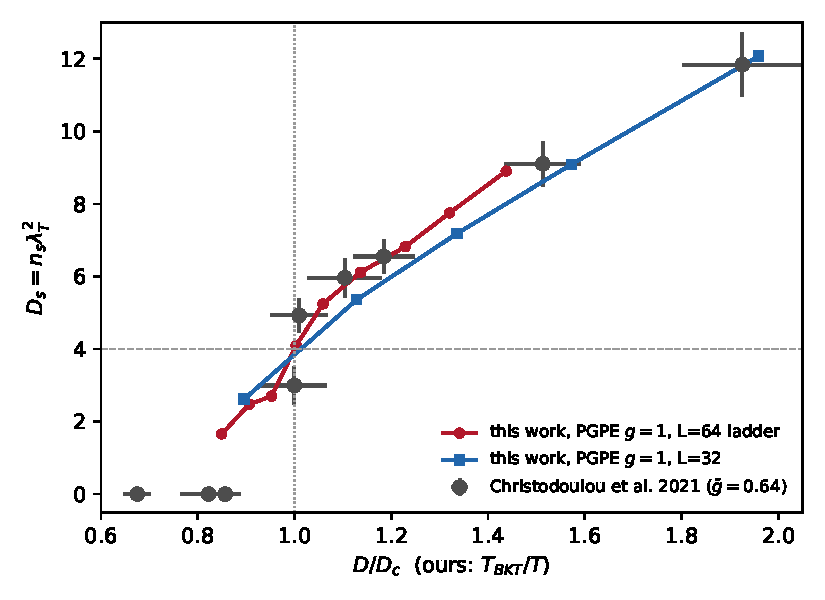
\includegraphics[width=0.62\textwidth]{figures/christodoulou_overlay.pdf}
\caption{Superfluid phase-space density against the reduced variable: Christodoulou et al.\ (points with
errors) and this programme's classical-field ladder and finite-size box, with $D/D_c$ identified with
$T_{\rm BKT}/T$. No parameter is adjusted.}\label{fig:overlay}
\end{figure}

\subsection{Thouless pumps as the existing matched pair}
Lohse et al.~\cite{Lohse2016} and Nakajima et al.~\cite{Nakajima2016}: a winding cycle pumps one
quantum per period, a non-winding cycle of the same drive pumps none. Cited as the paradigm; no new
analysis.

\section{What this proposal does not claim}
\begin{failbox}
\begin{itemize}[leftmargin=*]
\item Novelty of the two-temperature picture: it is Onsager's, and it is measured~\cite{Gauthier2019,
  Johnstone2019,Groszek2018}. Novelty of the mediant inequality: none; its value is that it is the
  exact statement, checked by two kernels, of why the round-2 thermometer clause was wrong in principle.
\item That the equipartition estimator reads $T_b$ exactly; this is what P1--P4 test.
\item Any transfer outside this system without its own matched intervention~\cite{Callens2026Astro}.
\end{itemize}
\end{failbox}

\bibliographystyle{unsrt}
\bibliography{refs_sector_temperature}
\end{document}
